\begin{flushleft}
\begin{figure}[!h]
    \centering
\begin{tabular}{|l|l|}
    \hline objet & quantité nécessaire  \\
    \hline câble élastique pour les articulations & 45cm/doigt\\
    \hline câble métal pour doigts & 54cm/doigt\\
    \hline super glue ou pistolet à colle chaude & environ 1 tube\\
    \hline vis & 14 (utiliser celles fournies avec les servomoteurs)\\
    \hline
\end{tabular}
\caption{Liste du matériel nécessaire au montage}
\label{fig:my_label}
\end{figure}
\end{flushleft}

\begin{flushleft}
\textbullet \, Positionner les différentes phalanges autour de la paume pour visualiser le résultat final :
\end{flushleft}

\begin{figure}[!h]
    \centering
    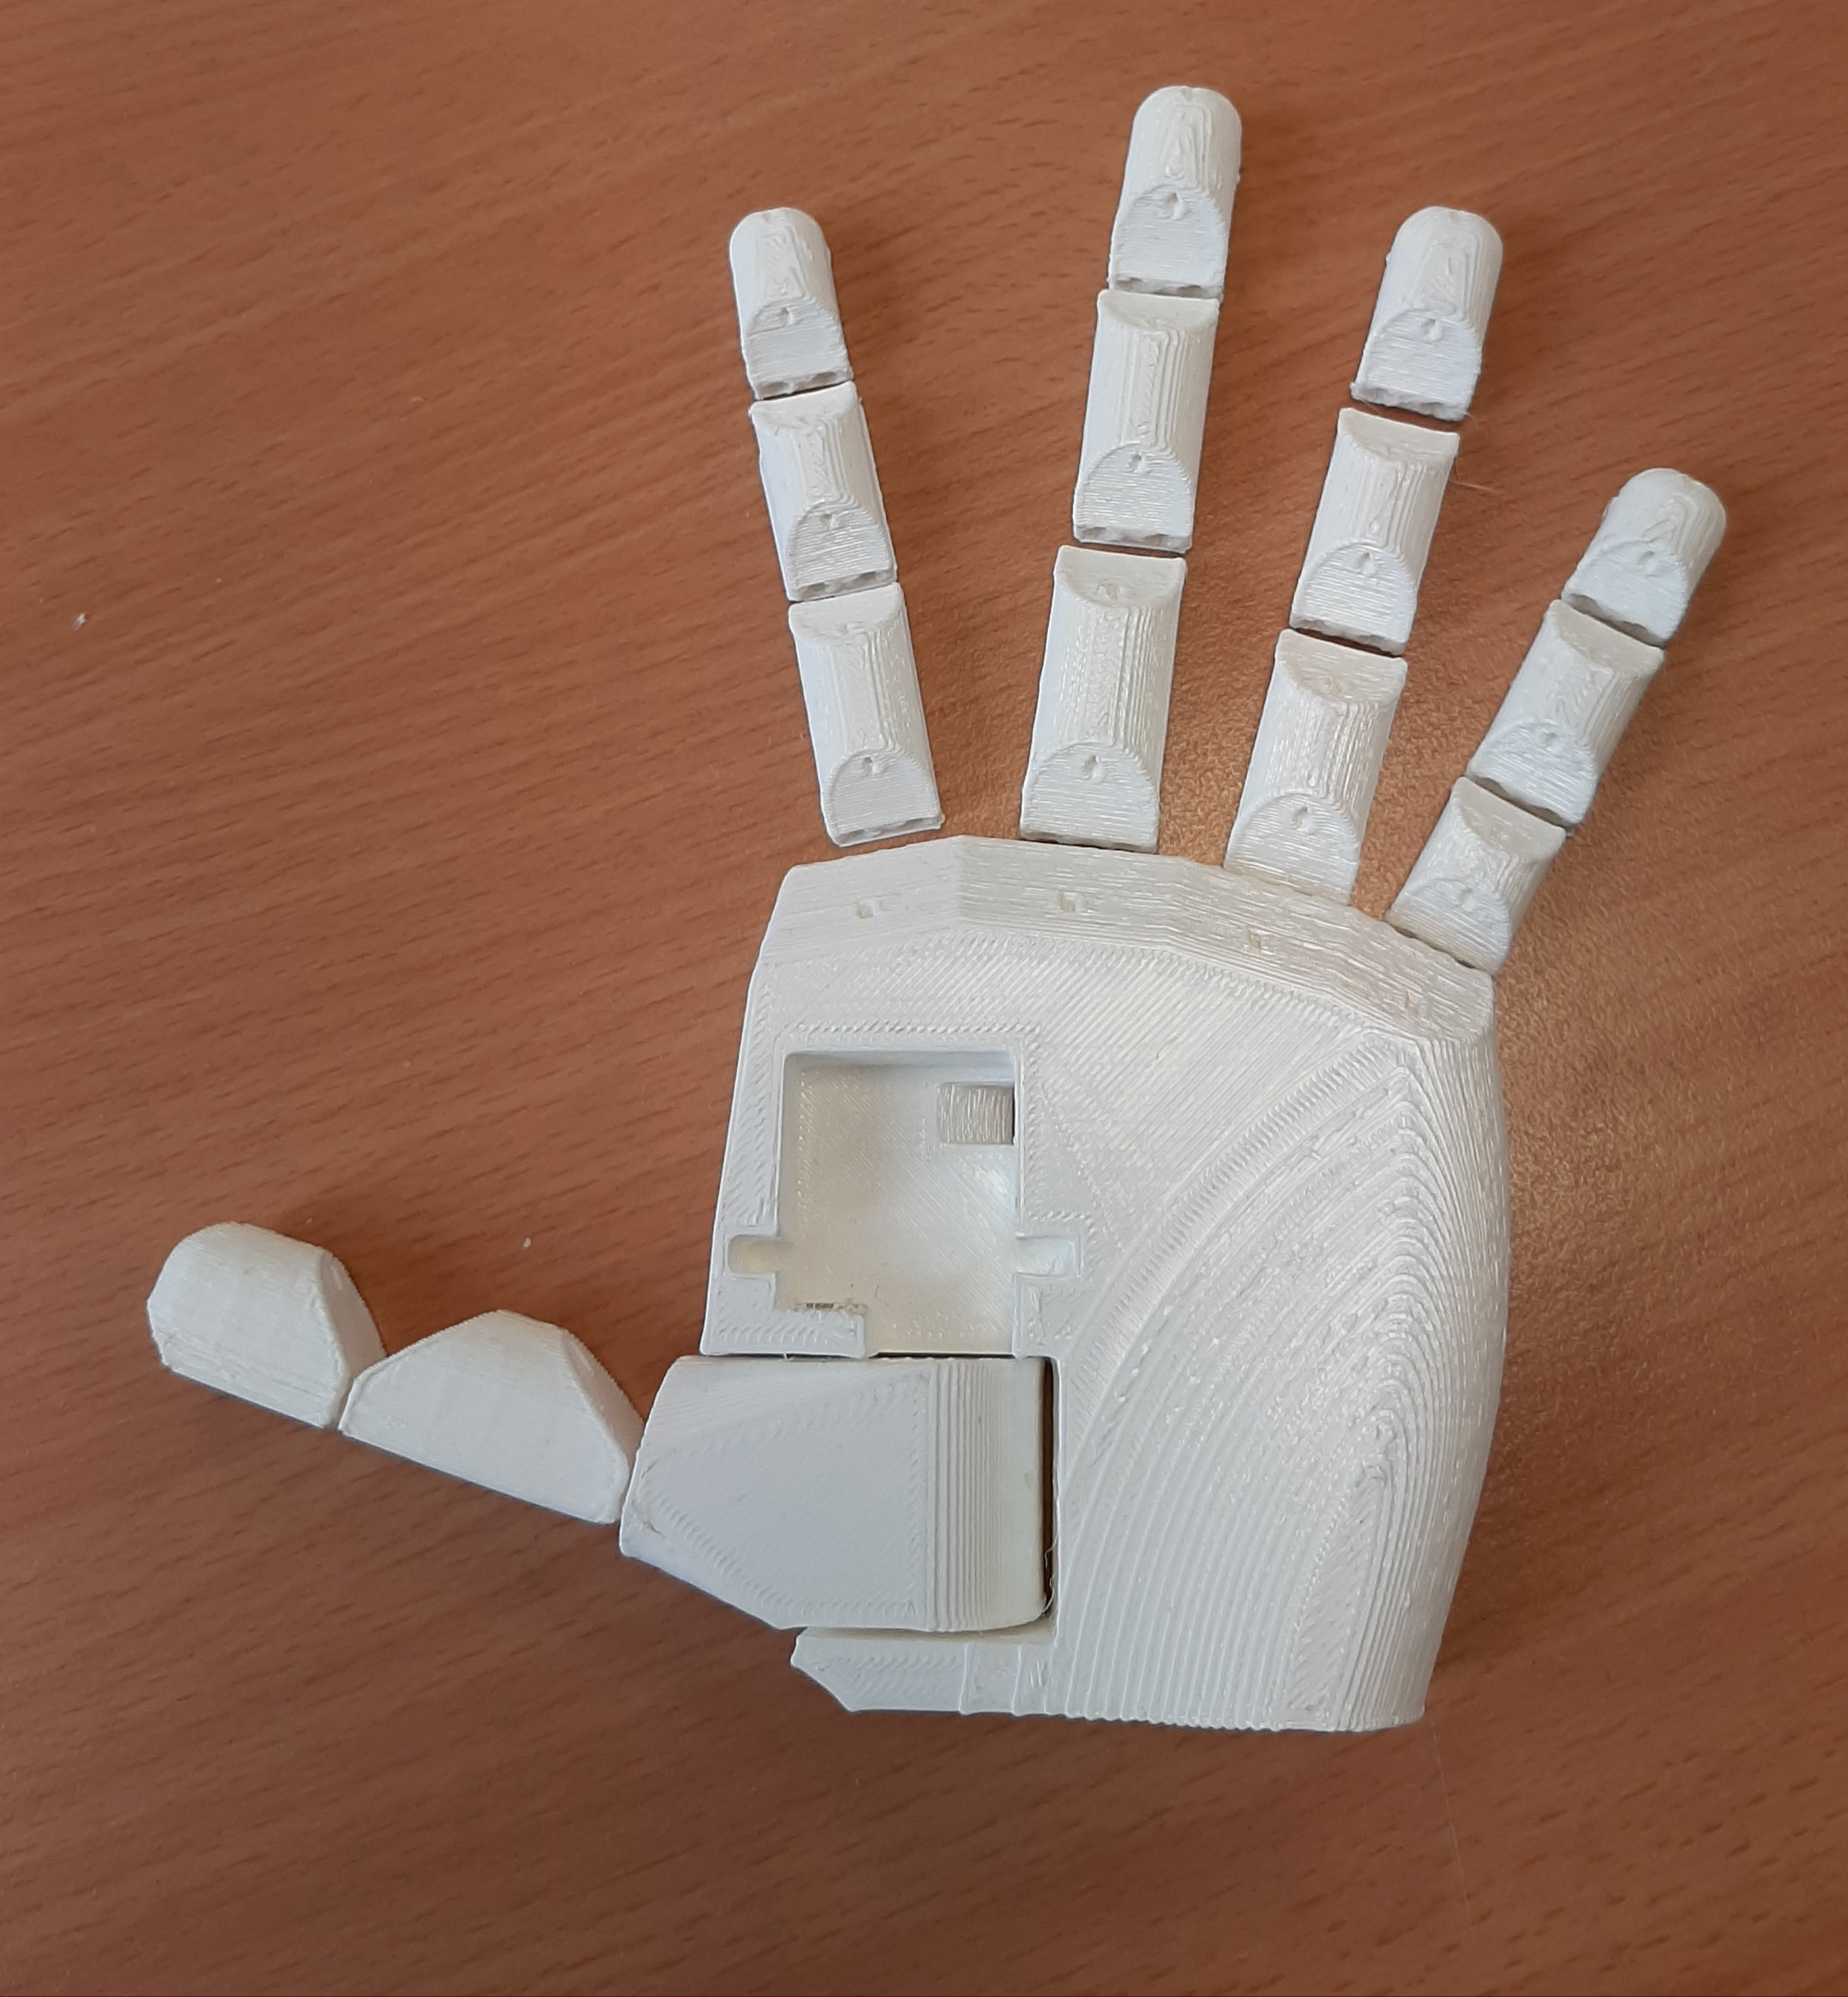
\includegraphics[width=400pt,height=400pt]{Déroulé/Jour_3/Montage de la main/étape 1.jpg}
    \caption{Montage de la main - \'Etape 1}
    \label{fig:my_label}
\end{figure}

%provisoire
\newpage

\begin{flushleft}
\textbullet \, Passer le câble souple une 1ère fois dans les différentes articulations des doigts puis dans la paume, et faire un 2ème tour si nécessaire pour que le fil soit plus tendu :
\end{flushleft}

\begin{figure}[!h]
    \centering
    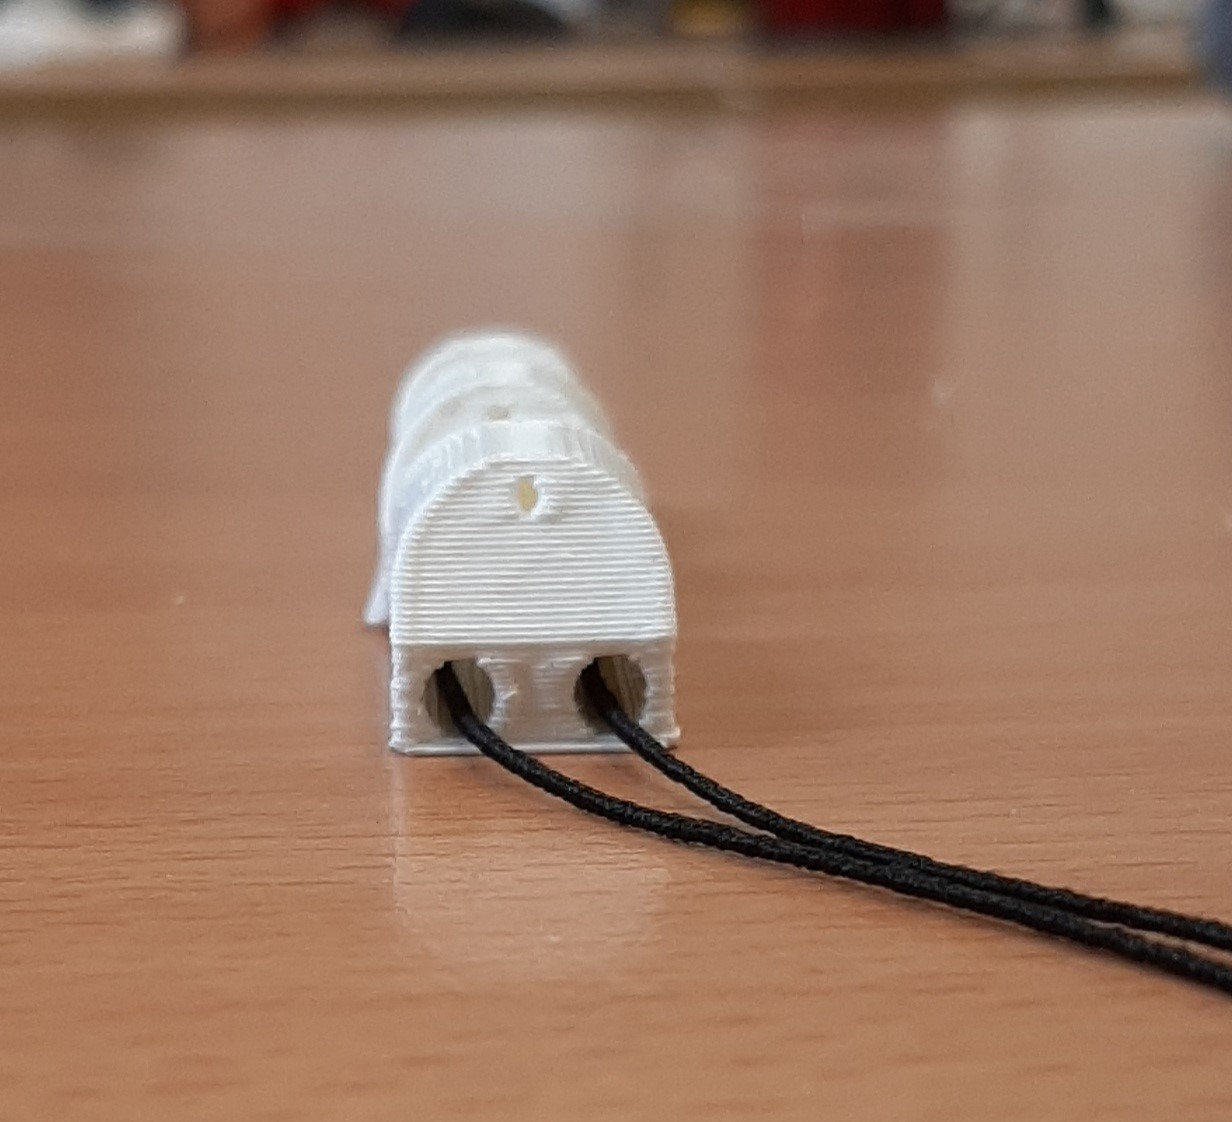
\includegraphics[width=200pt, height=200pt]{Déroulé/Jour_3/Montage de la main/étape2_1.jpg}
    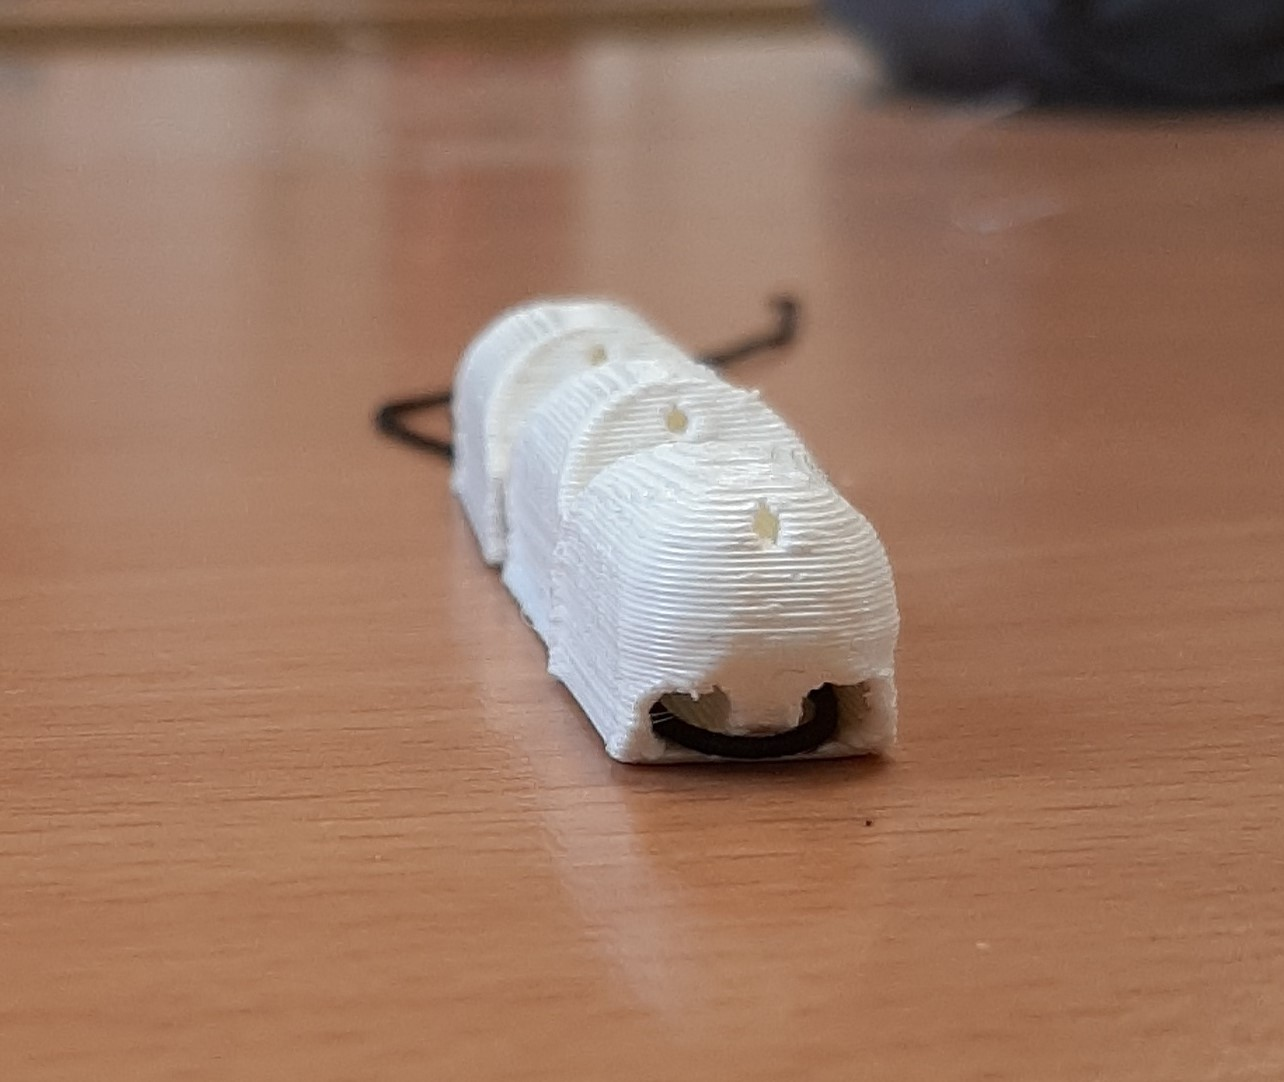
\includegraphics[width=200pt, height=200pt]{Déroulé/Jour_3/Montage de la main/étape2_2.jpg}
    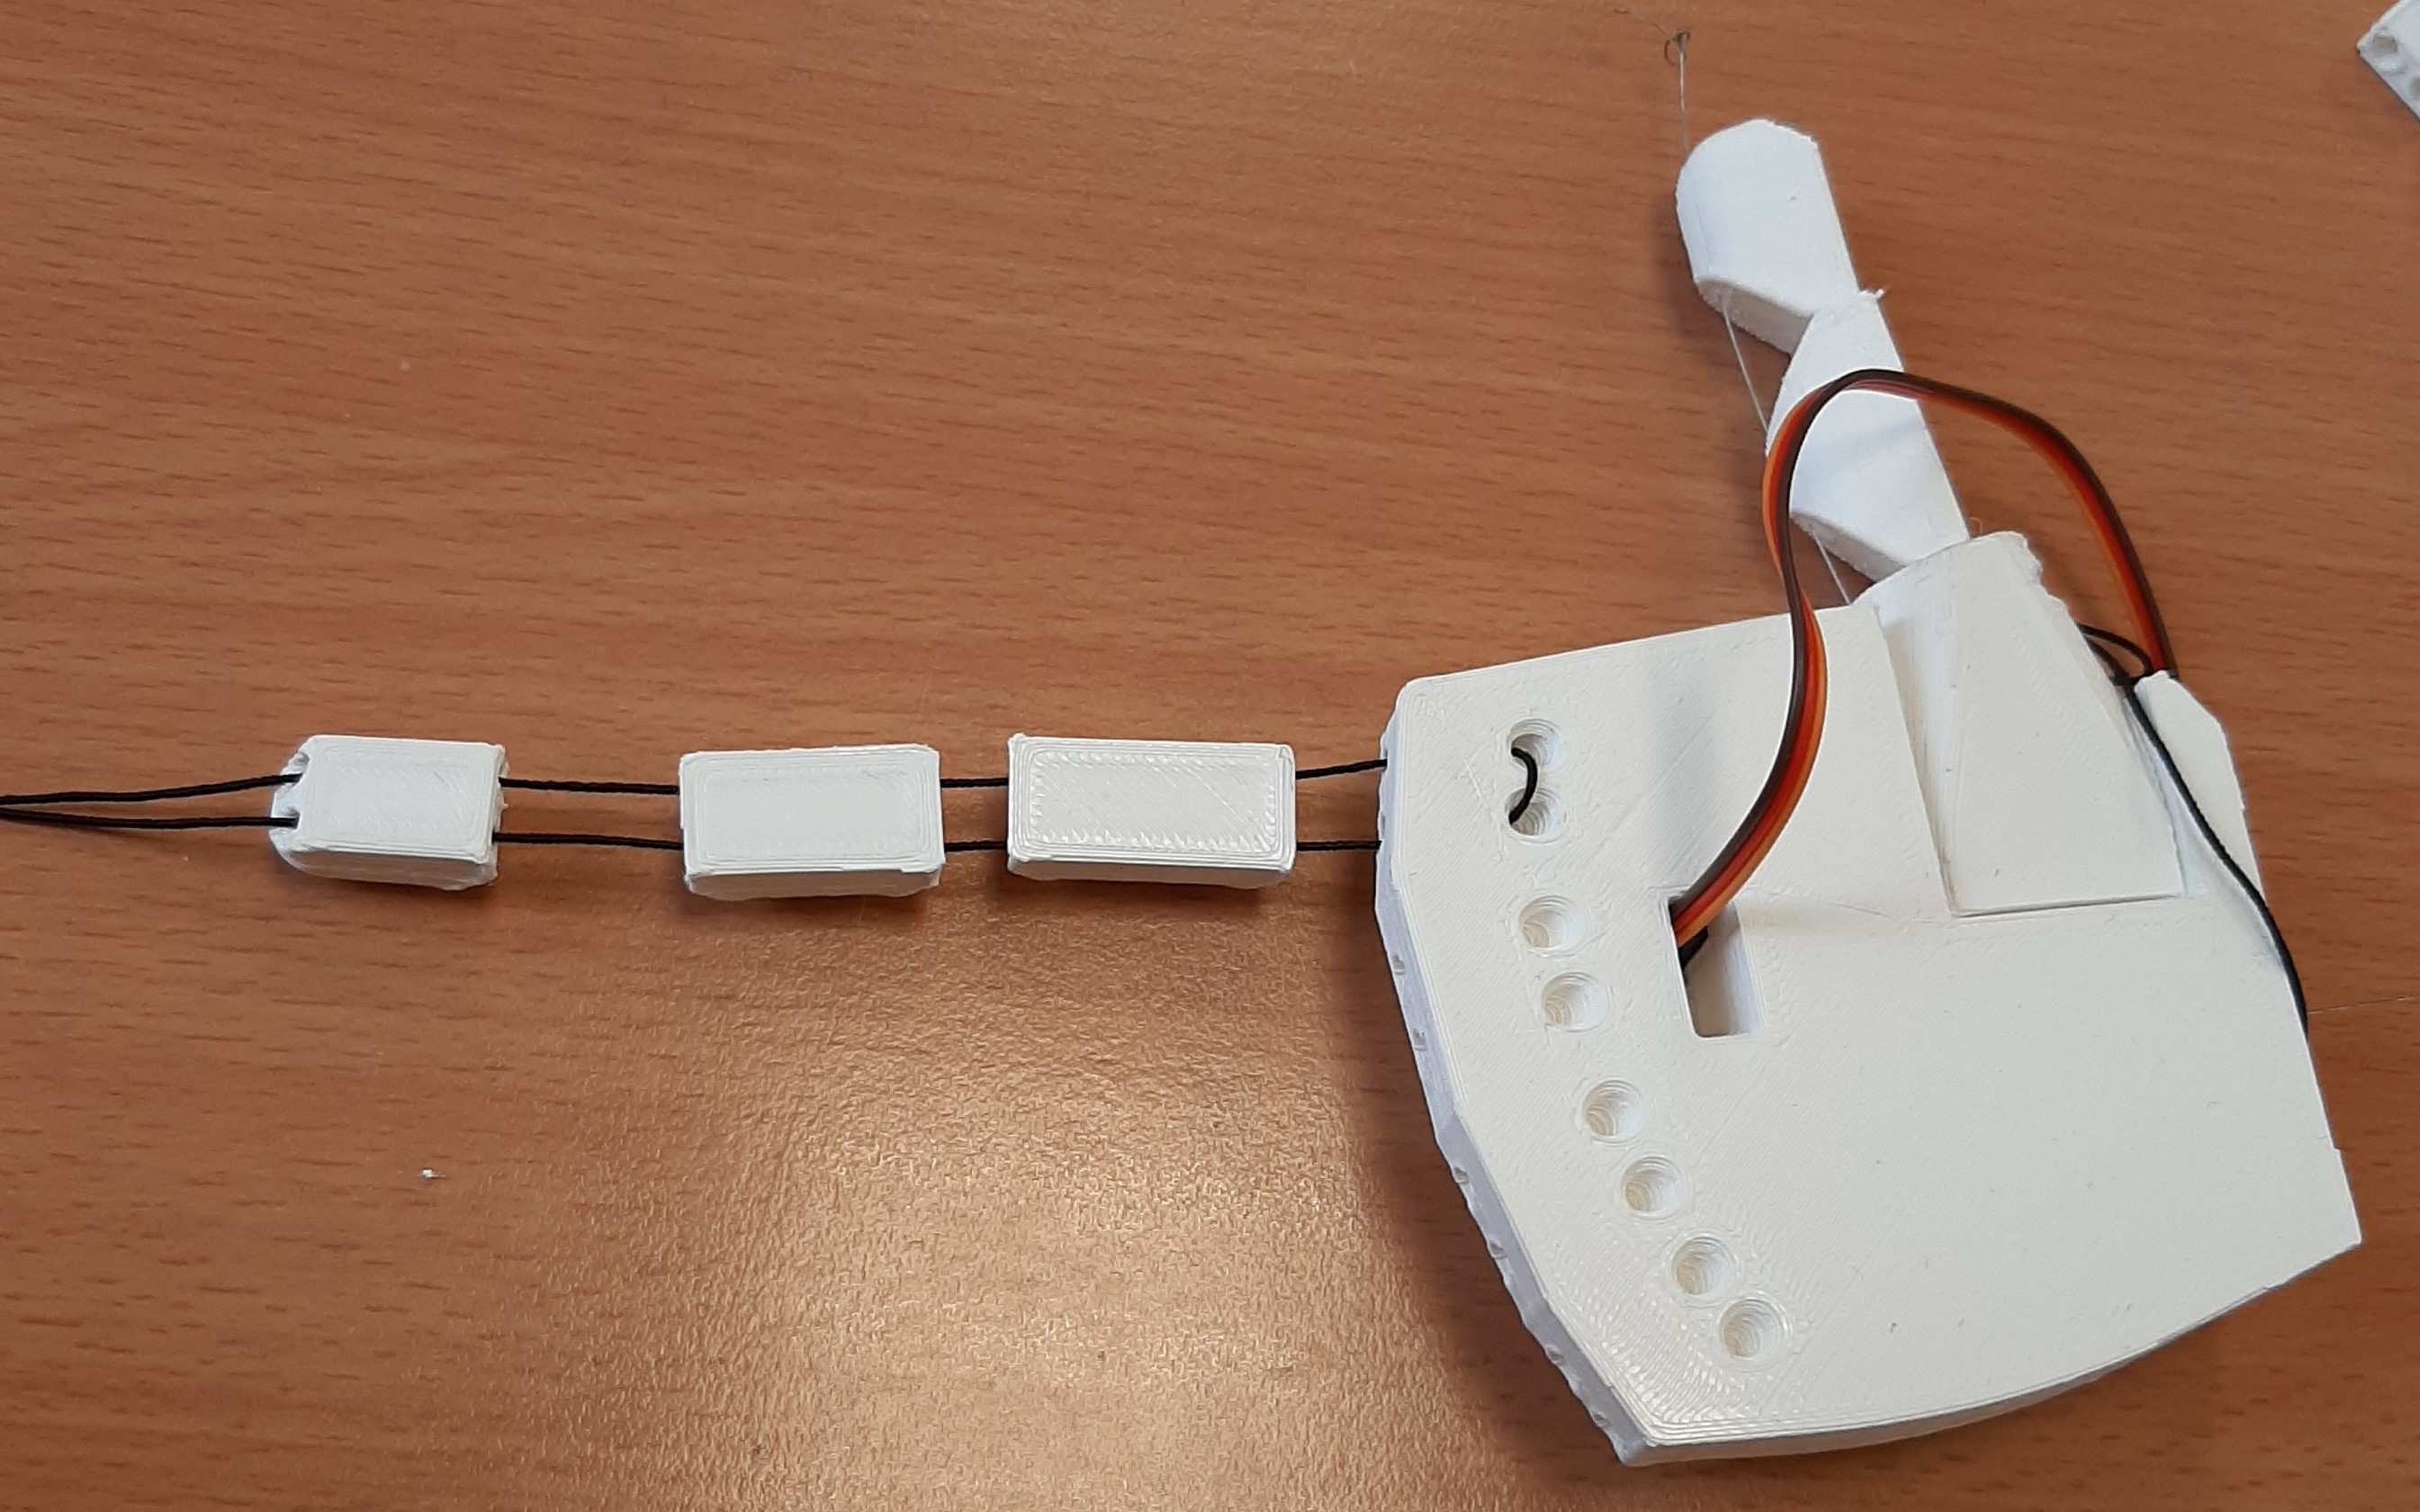
\includegraphics[width=250pt, height=200pt]{Déroulé/Jour_3/Montage de la main/étape2_3.jpg}
    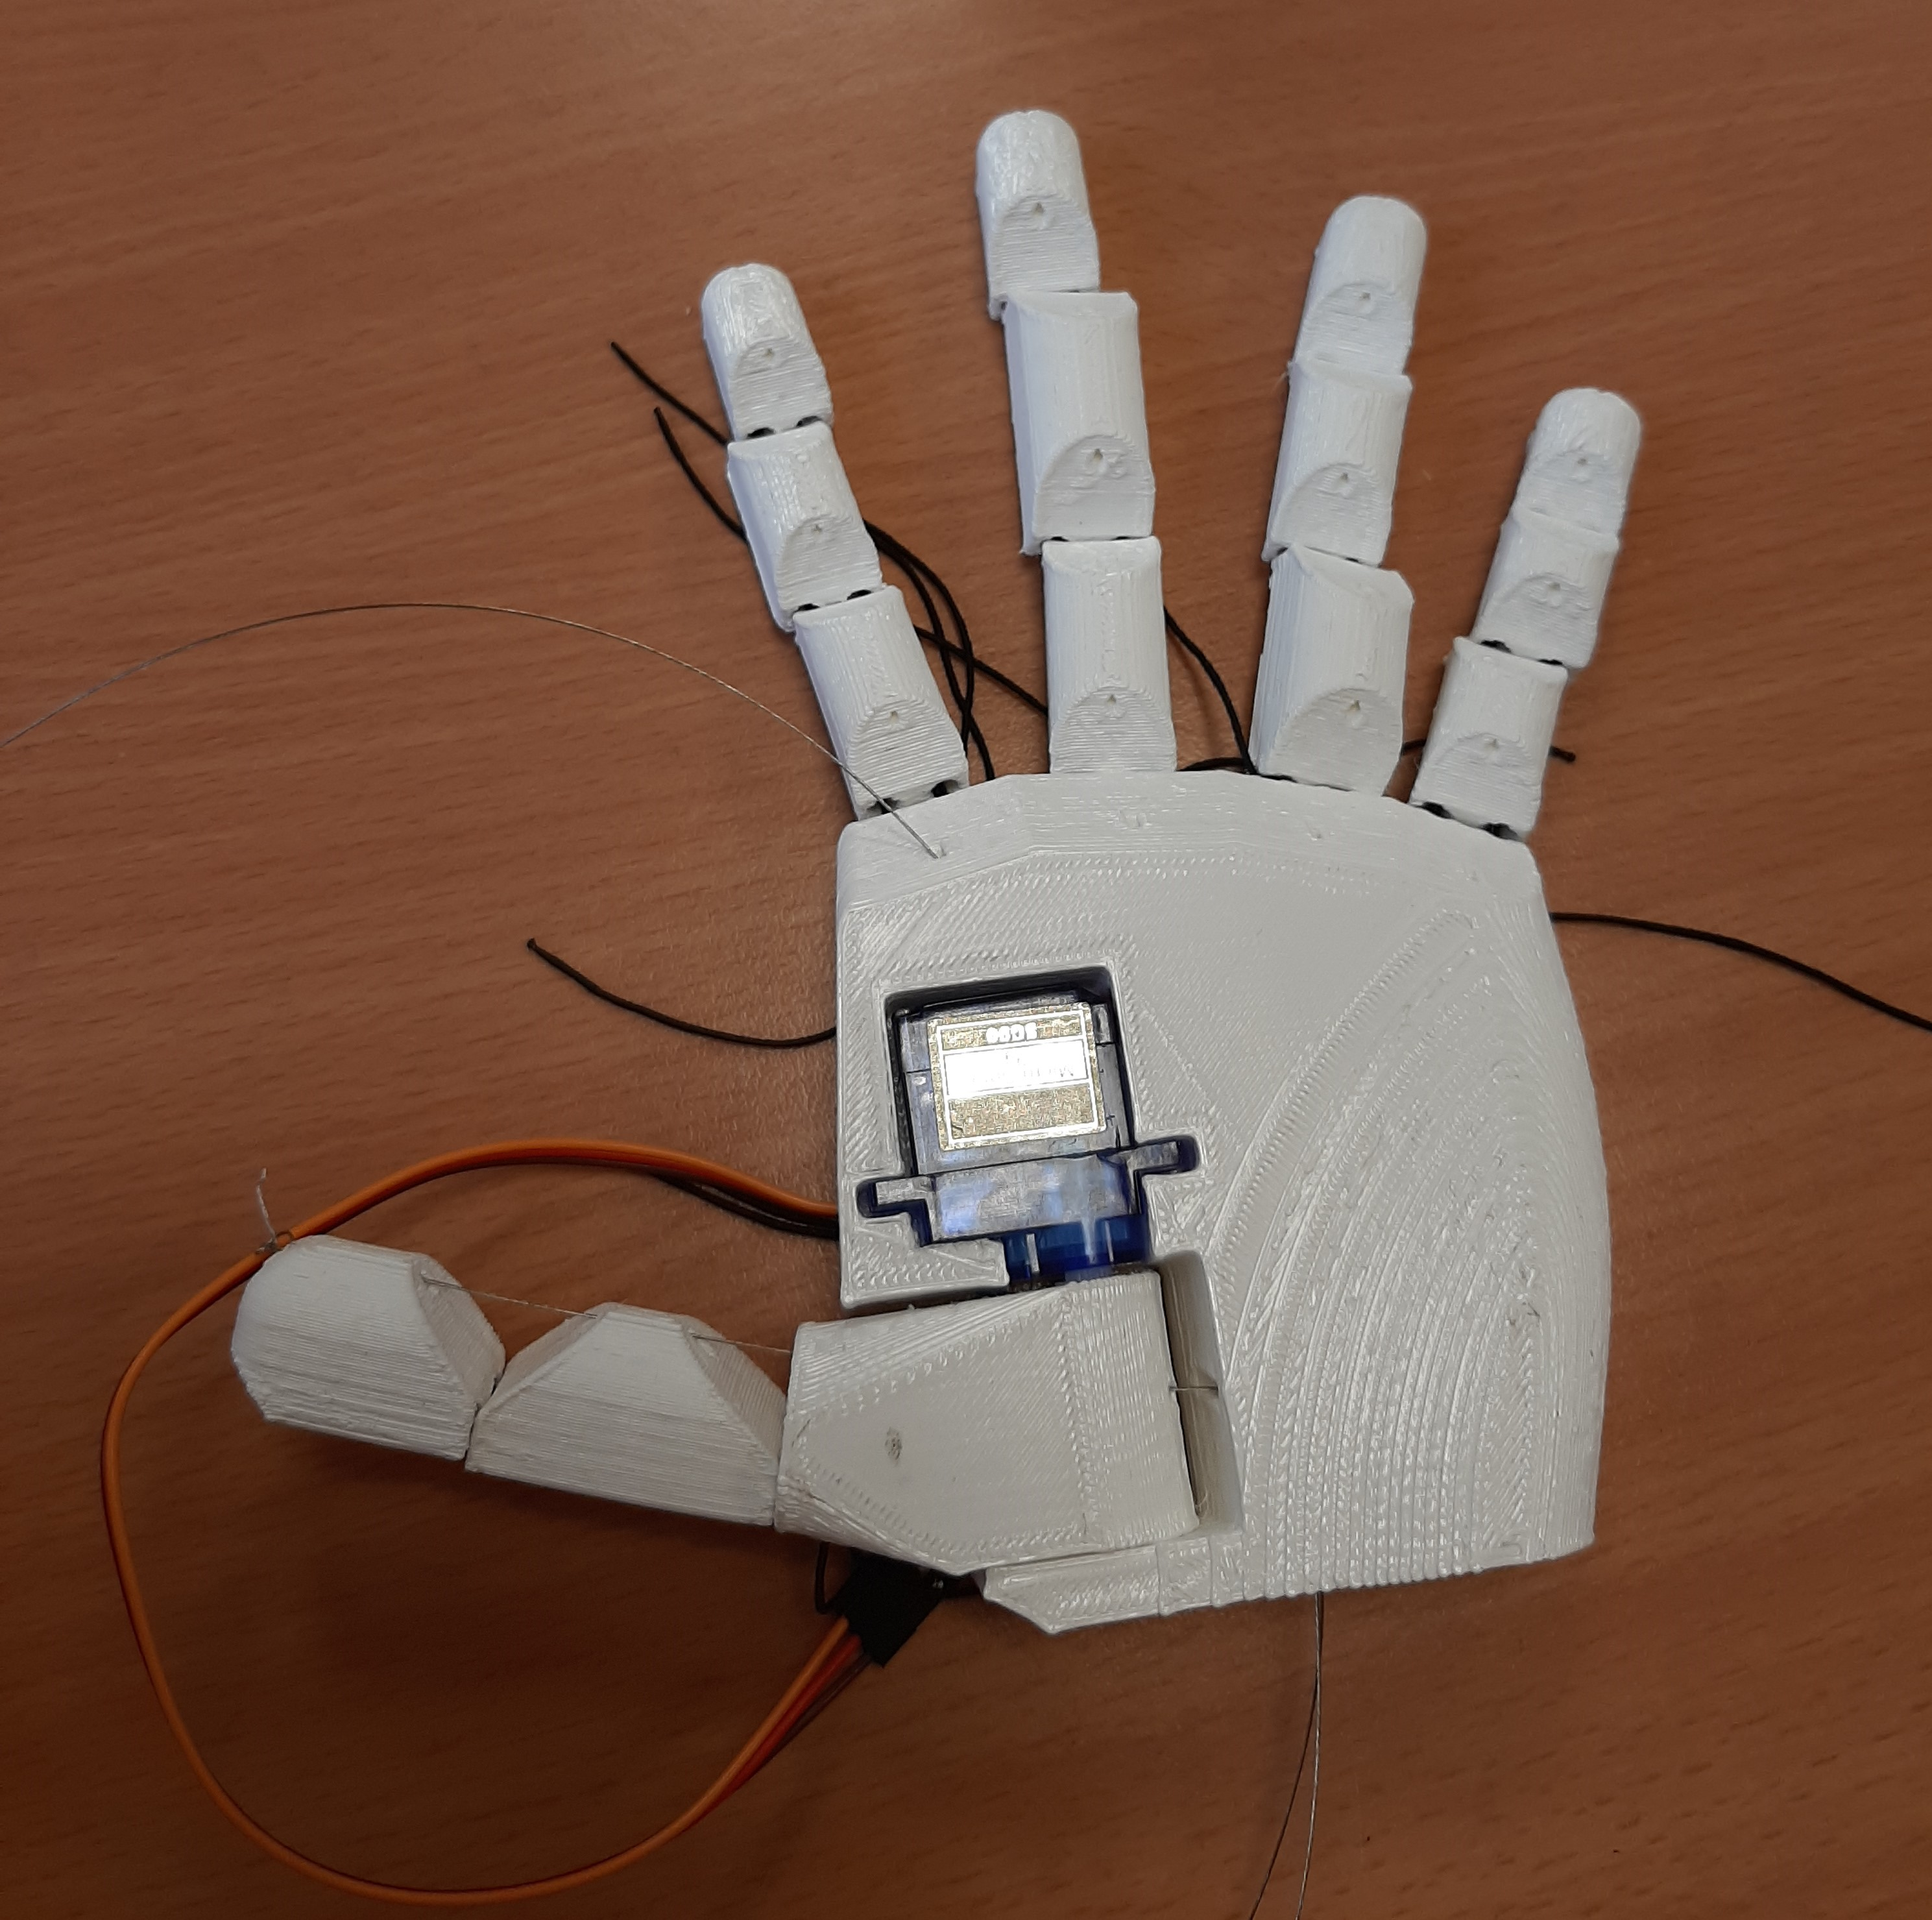
\includegraphics[width=200pt, height=200pt]{Déroulé/Jour_3/Montage de la main/étape2_4.jpg}
    \caption[\'Etape 2]{Montage de la main - \'Etape 2}
    \label{fig:my_label}
\end{figure}

%provisoire
\newpage

\begin{flushleft}
\textbullet \, Visser sur la poulie le petit palonnier en utilisant la petite vis à l'extremité et l'une des grandes au centre :

\begin{figure}[!h]
    \centering
    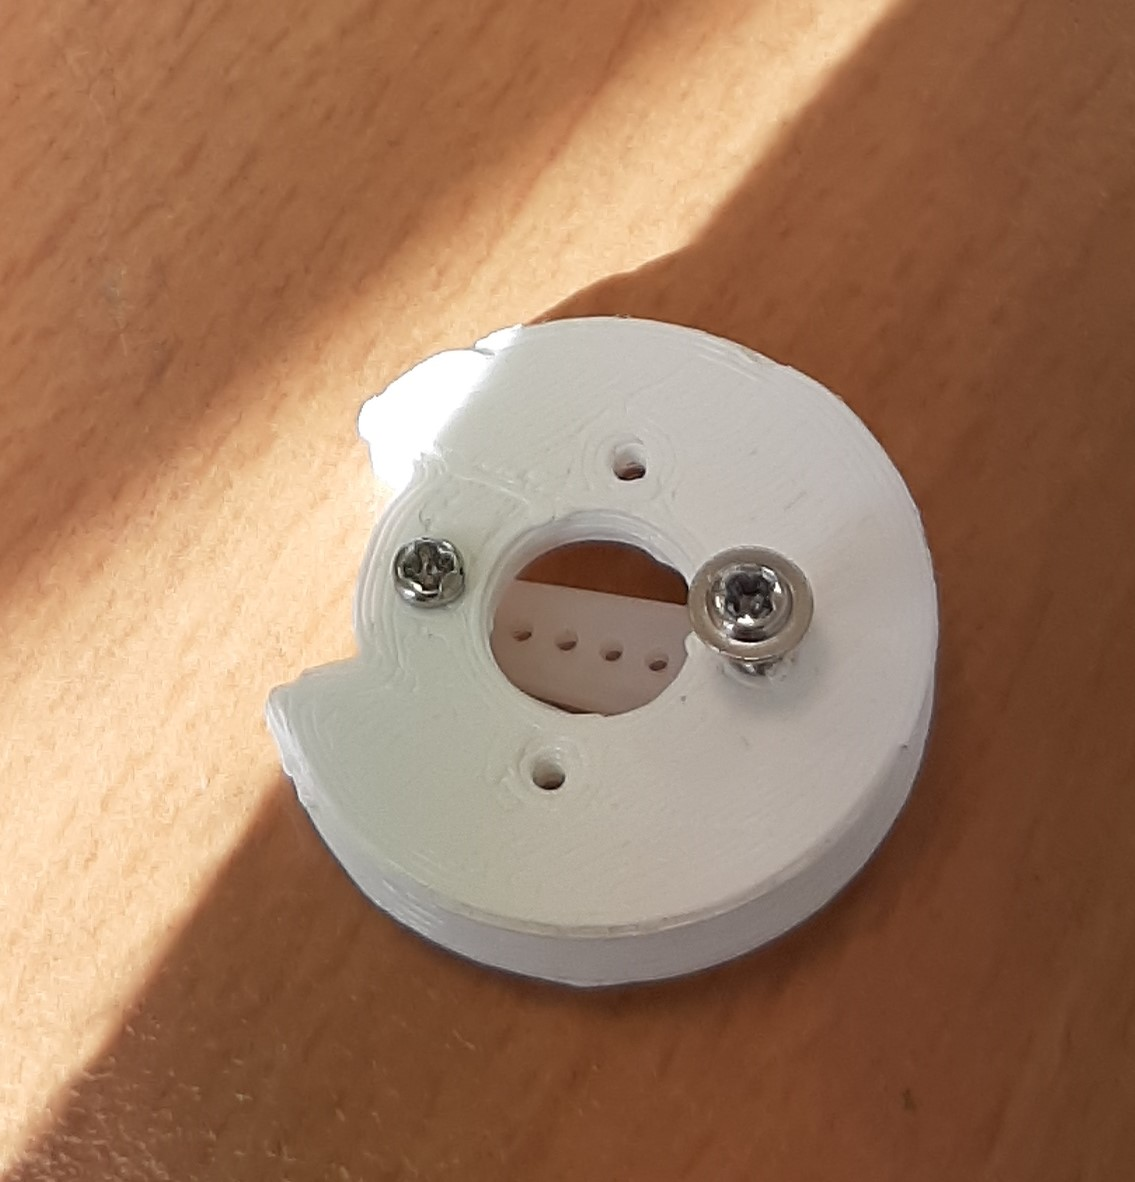
\includegraphics[width=200pt]{Déroulé/Jour_3/Montage de la main/étape3_1.jpg}
    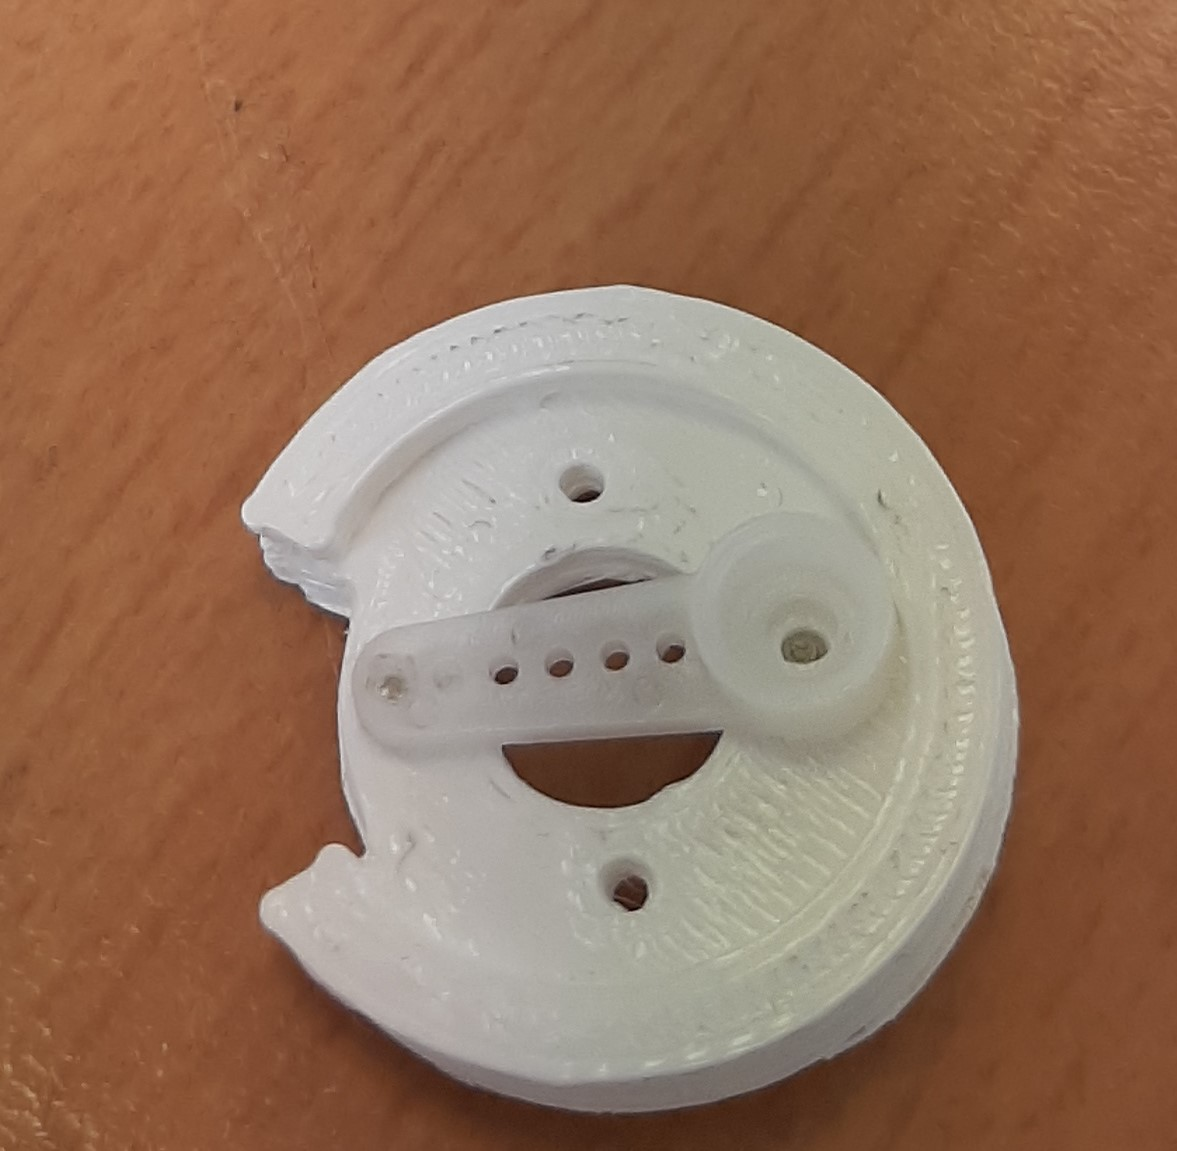
\includegraphics[width=200pt]{Déroulé/Jour_3/Montage de la main/étape3_2.jpg}
    \caption[\'Etape 3]{Montage de la main - \'Etape 3}
    \label{fig:my_label}
\end{figure}

\begin{multicols}{2}
        
\includegraphics[width=60pt,height=60pt]{Déroulé/Jour_1/Manuel d'utilisation/Images/6.jpg}
    
        \columnbreak
    
        \textbf{\large Attention : }\textbf{\textit{ Ne pas visser entièrement la grande vis.}}\\\vspace{0.2cm}
\end{multicols}

\textbullet \, Finir de fixer la grosse vis dans au centre de l'engrenage du servomoteur :

\begin{figure}[!h]
    \centering
    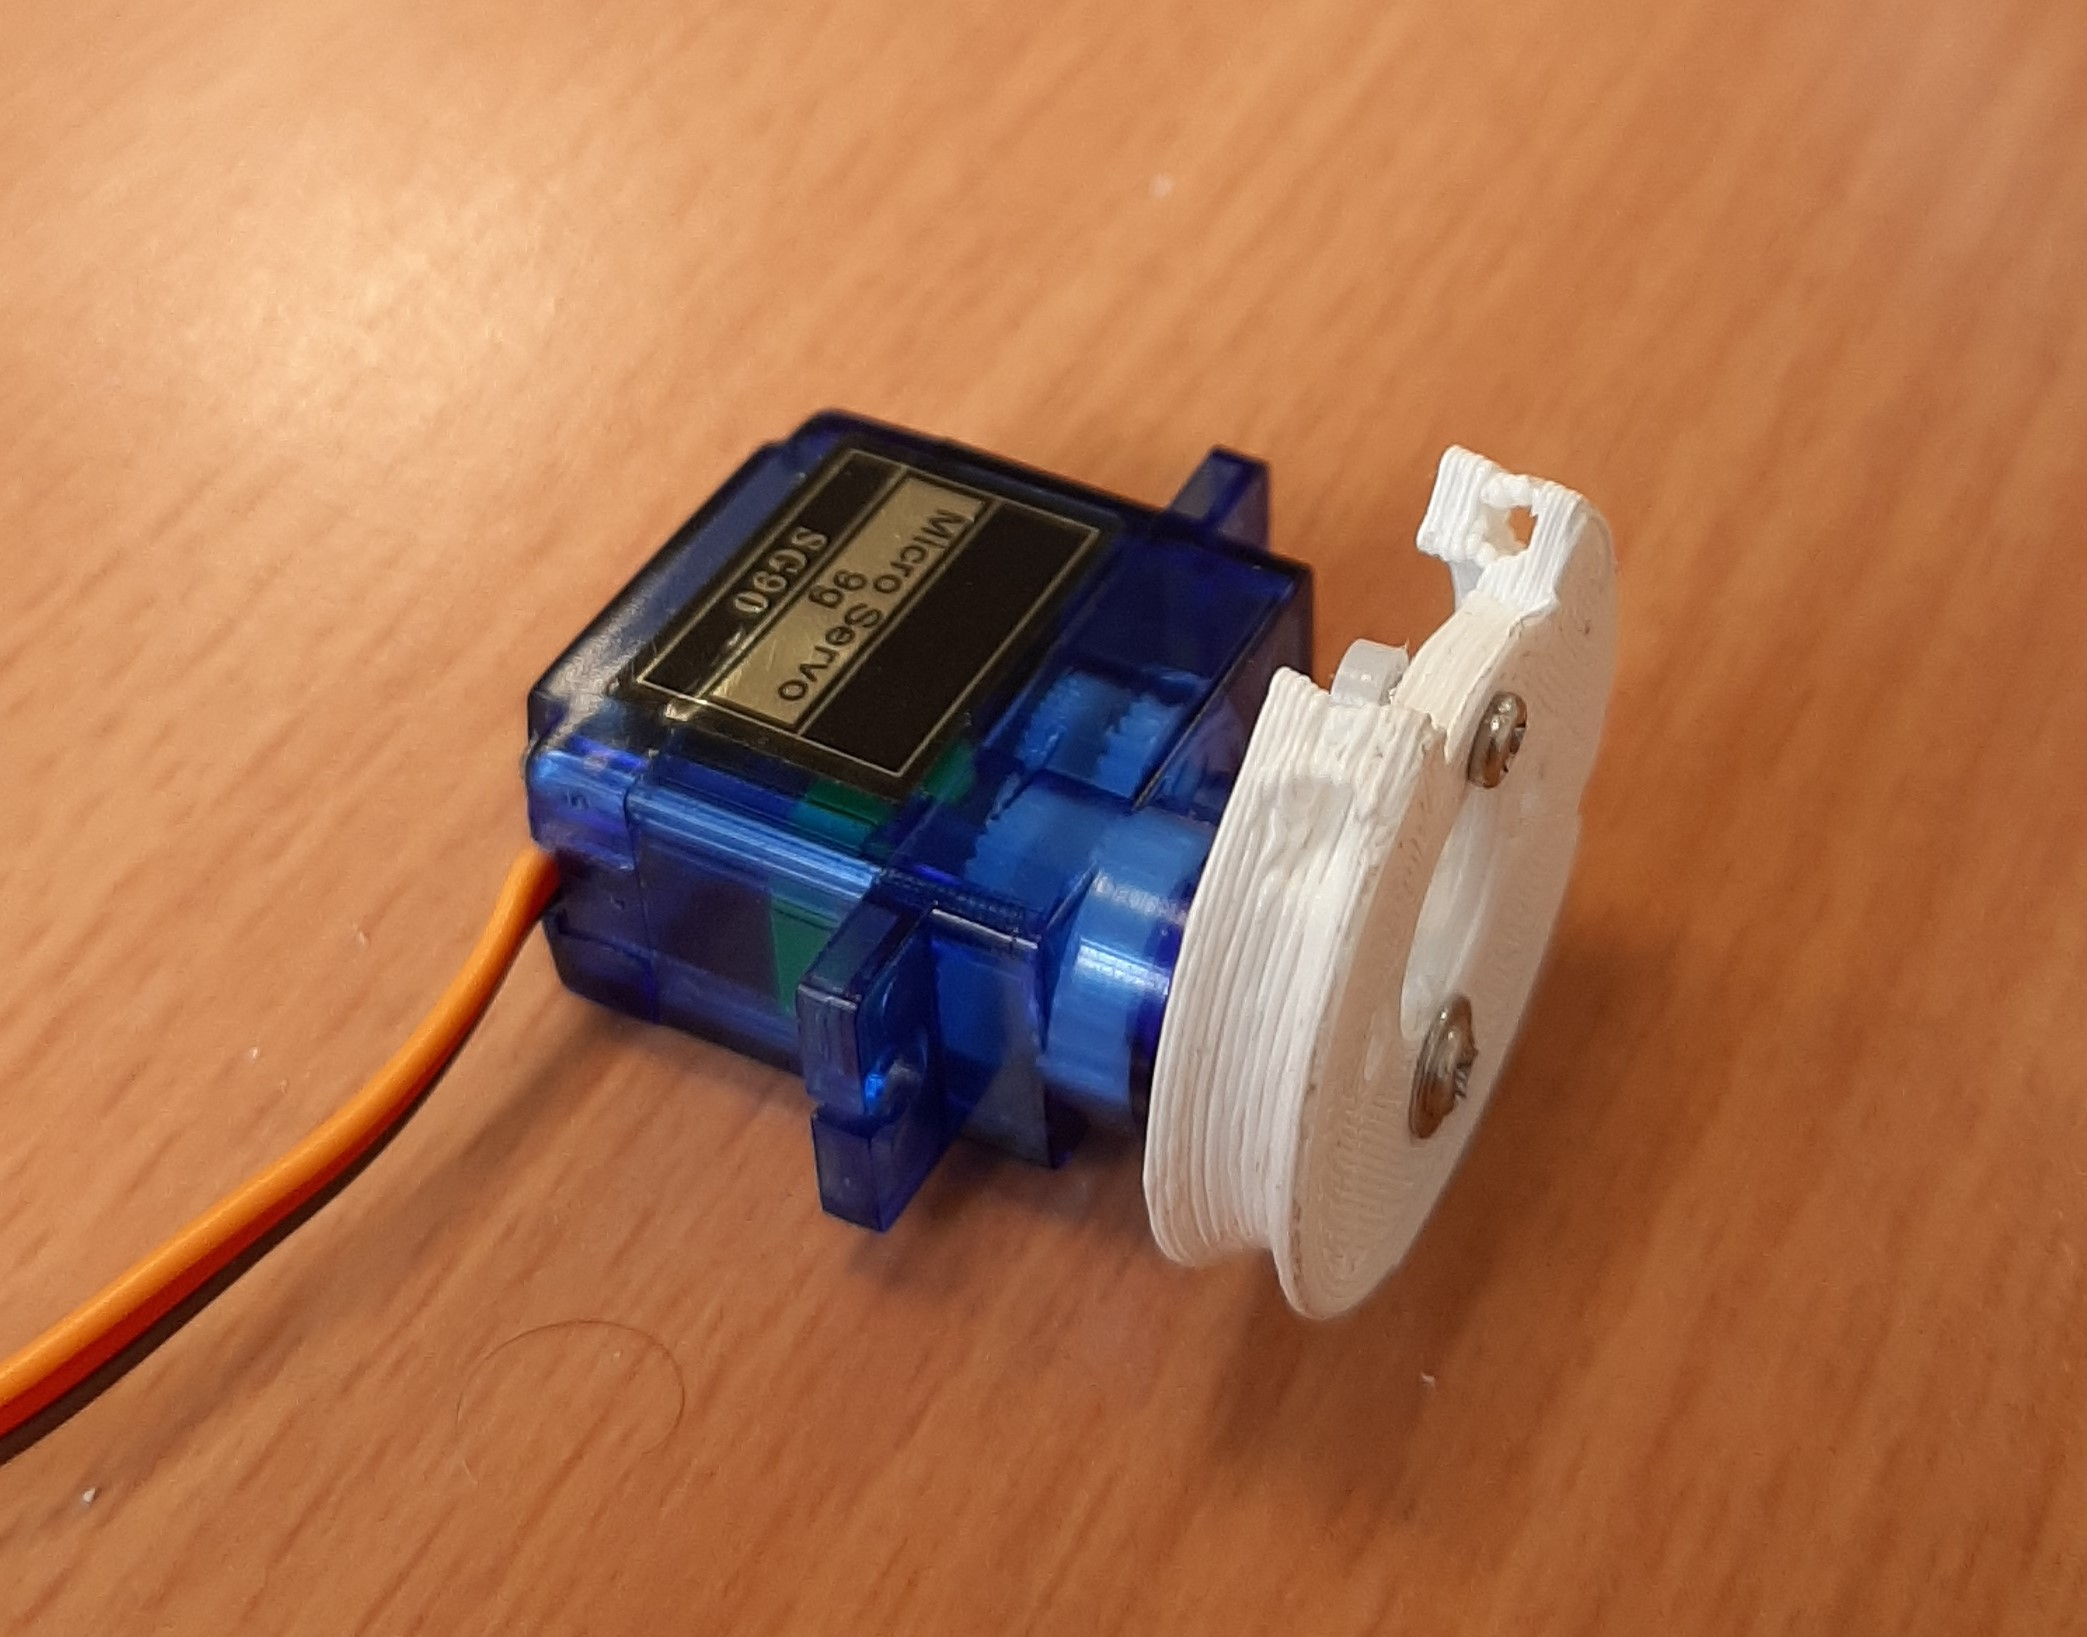
\includegraphics[width=300pt]{Déroulé/Jour_3/Montage de la main/étape4.jpg}
    \caption[\'Etape 4]{Montage de la main - \'Etape 4}
    \label{fig:my_label}
\end{figure}

\begin{multicols}{2}
        
\includegraphics[width=60pt,height=60pt]{Déroulé/Jour_1/Manuel d'utilisation/Images/6.jpg}
    
        \columnbreak
    
        \textbf{\large Attention : }\textbf{\textit{ Les servomoteurs que nous utilisons ont une course de 180°, il faut donc positionner correctement le palonnier avant de visser pour ne pas faire forcer le servomoteur lors du fonctionnement.}}\\\vspace{0.2cm}
\end{multicols}

\textbullet \, Fixer les servomoteurs sur le support. Pour cela utiliser la grand vis restante dans le sachet du servomoteur. Des trous sont présents sur le support :

\begin{figure}[!h]
    \centering
    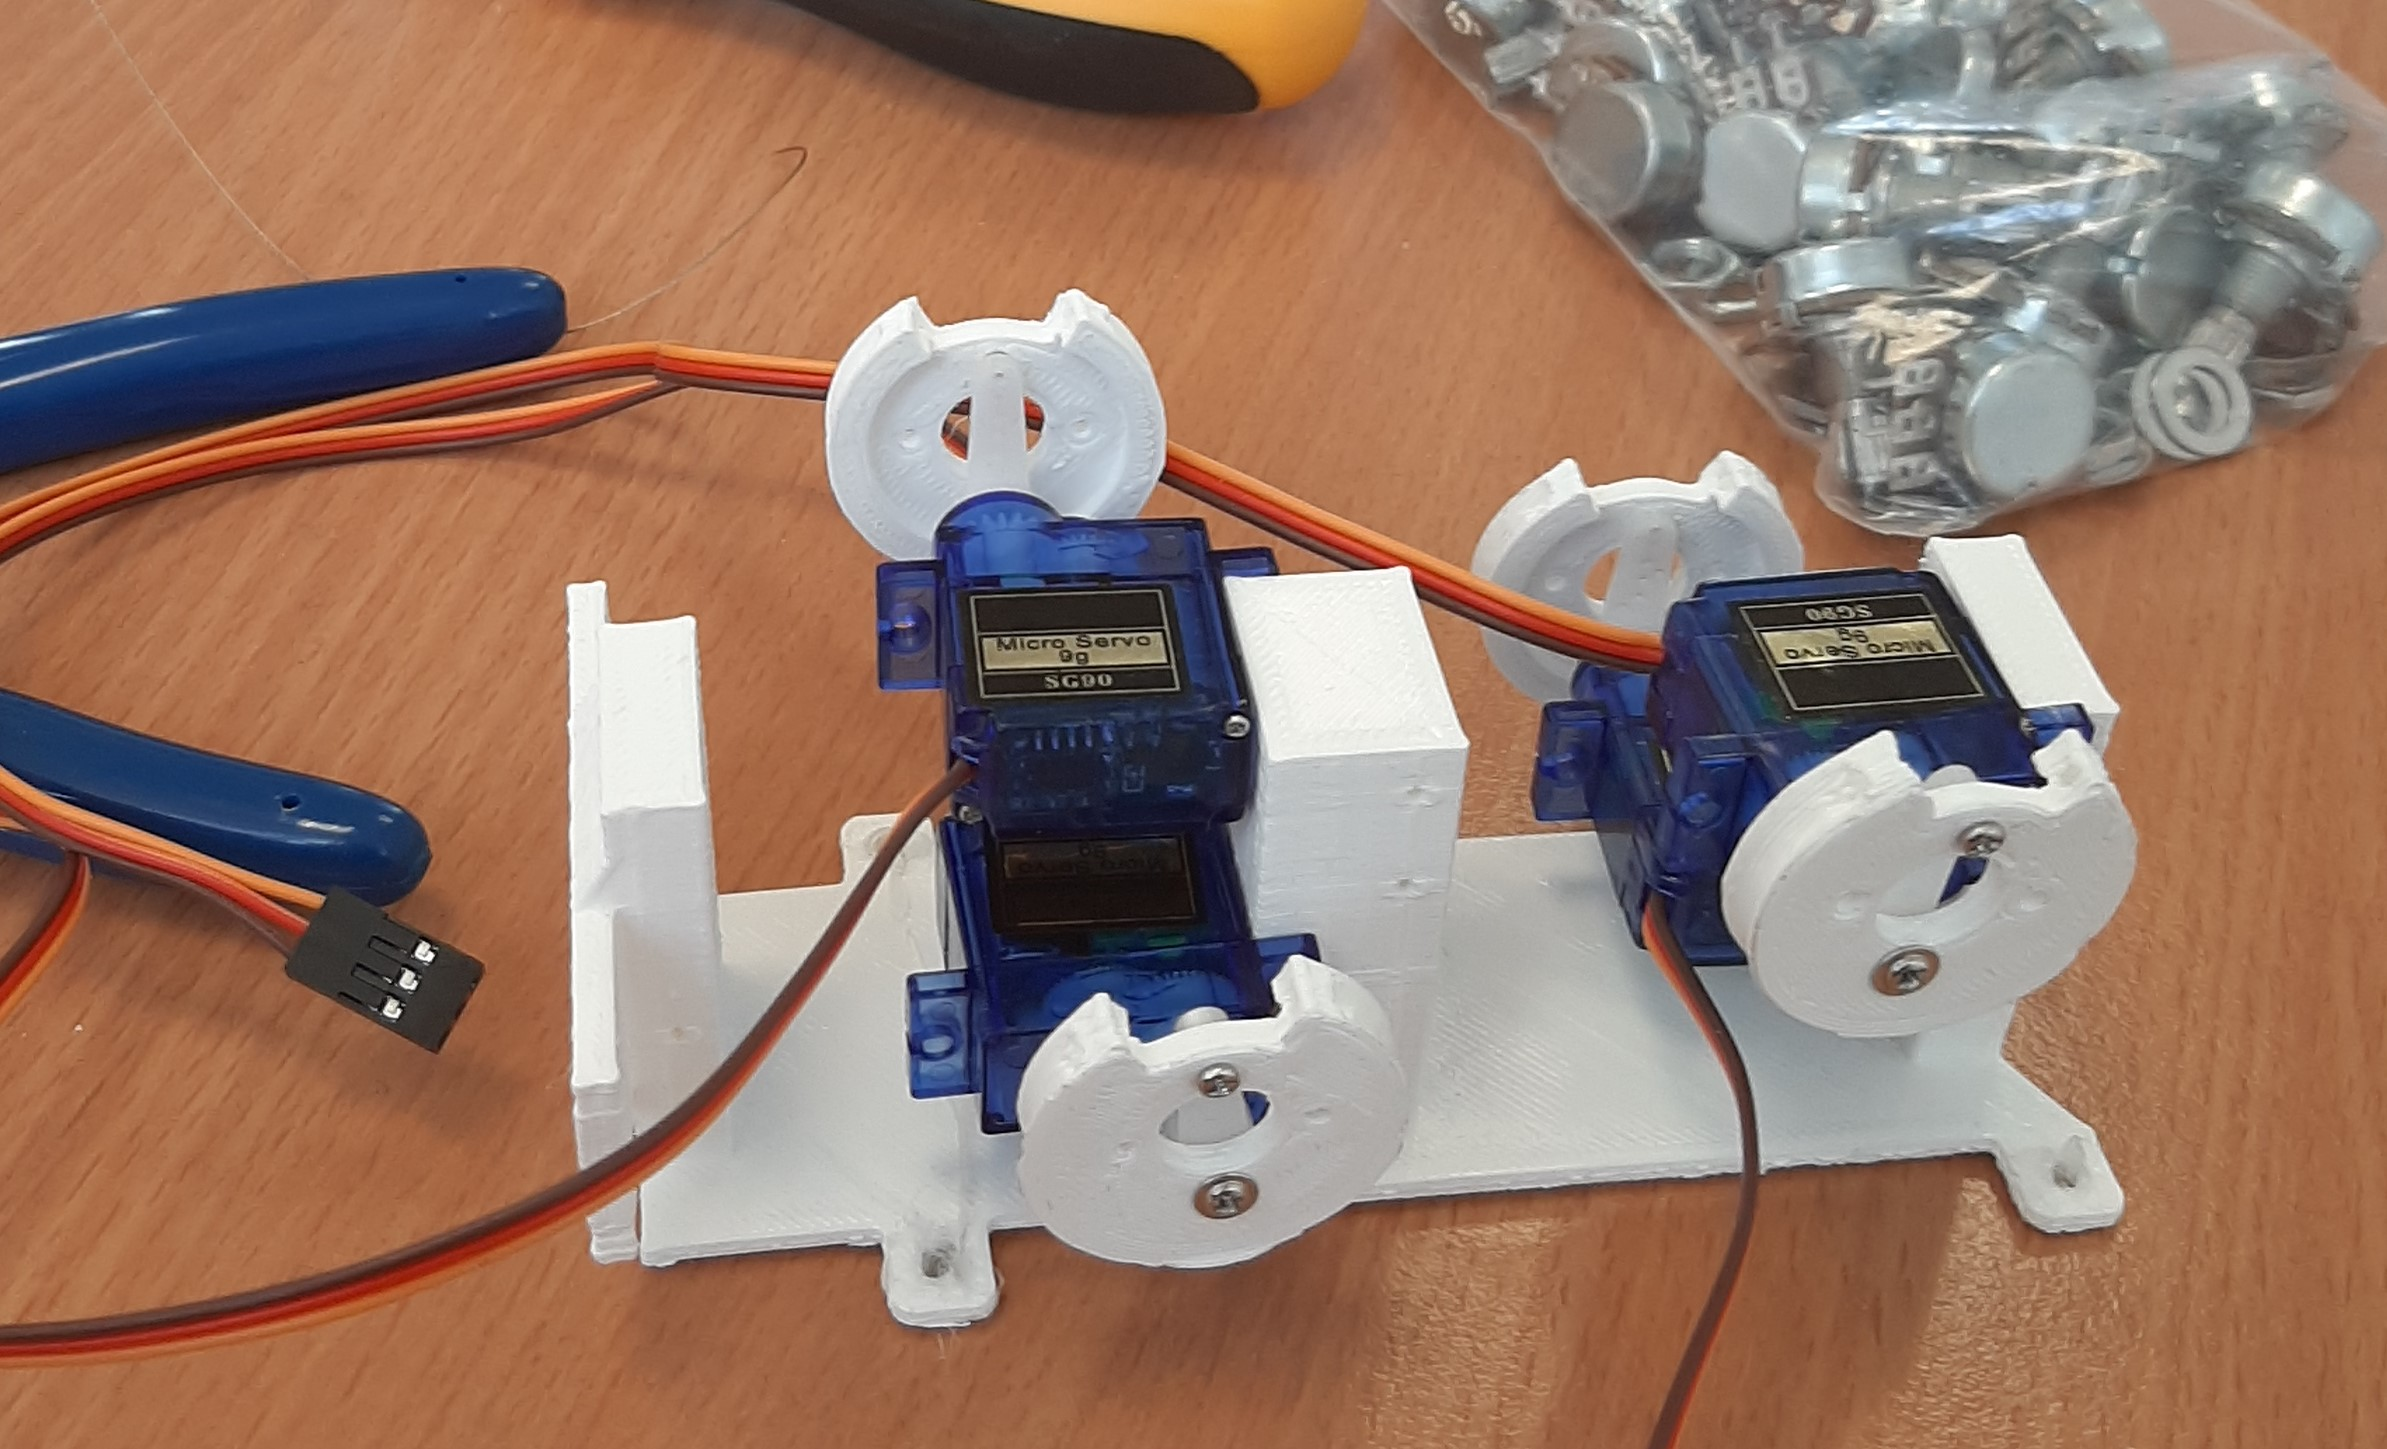
\includegraphics[width=300pt]{Déroulé/Jour_3/Montage de la main/étape5.jpg}
    \caption[\'Etape 5]{Montage de la main - \'Etape 5}
    \label{fig:my_label}
\end{figure}

%provisoire
\newpage

\textbullet \, Fixer le support à l'intérieur de l'avant bras, enrouler les câbles des doigts au niveau des poulies et câbler les potentiomètres et les servomoteurs sur votre breadboard et votre carte :

\begin{figure}[!h]
    \centering
    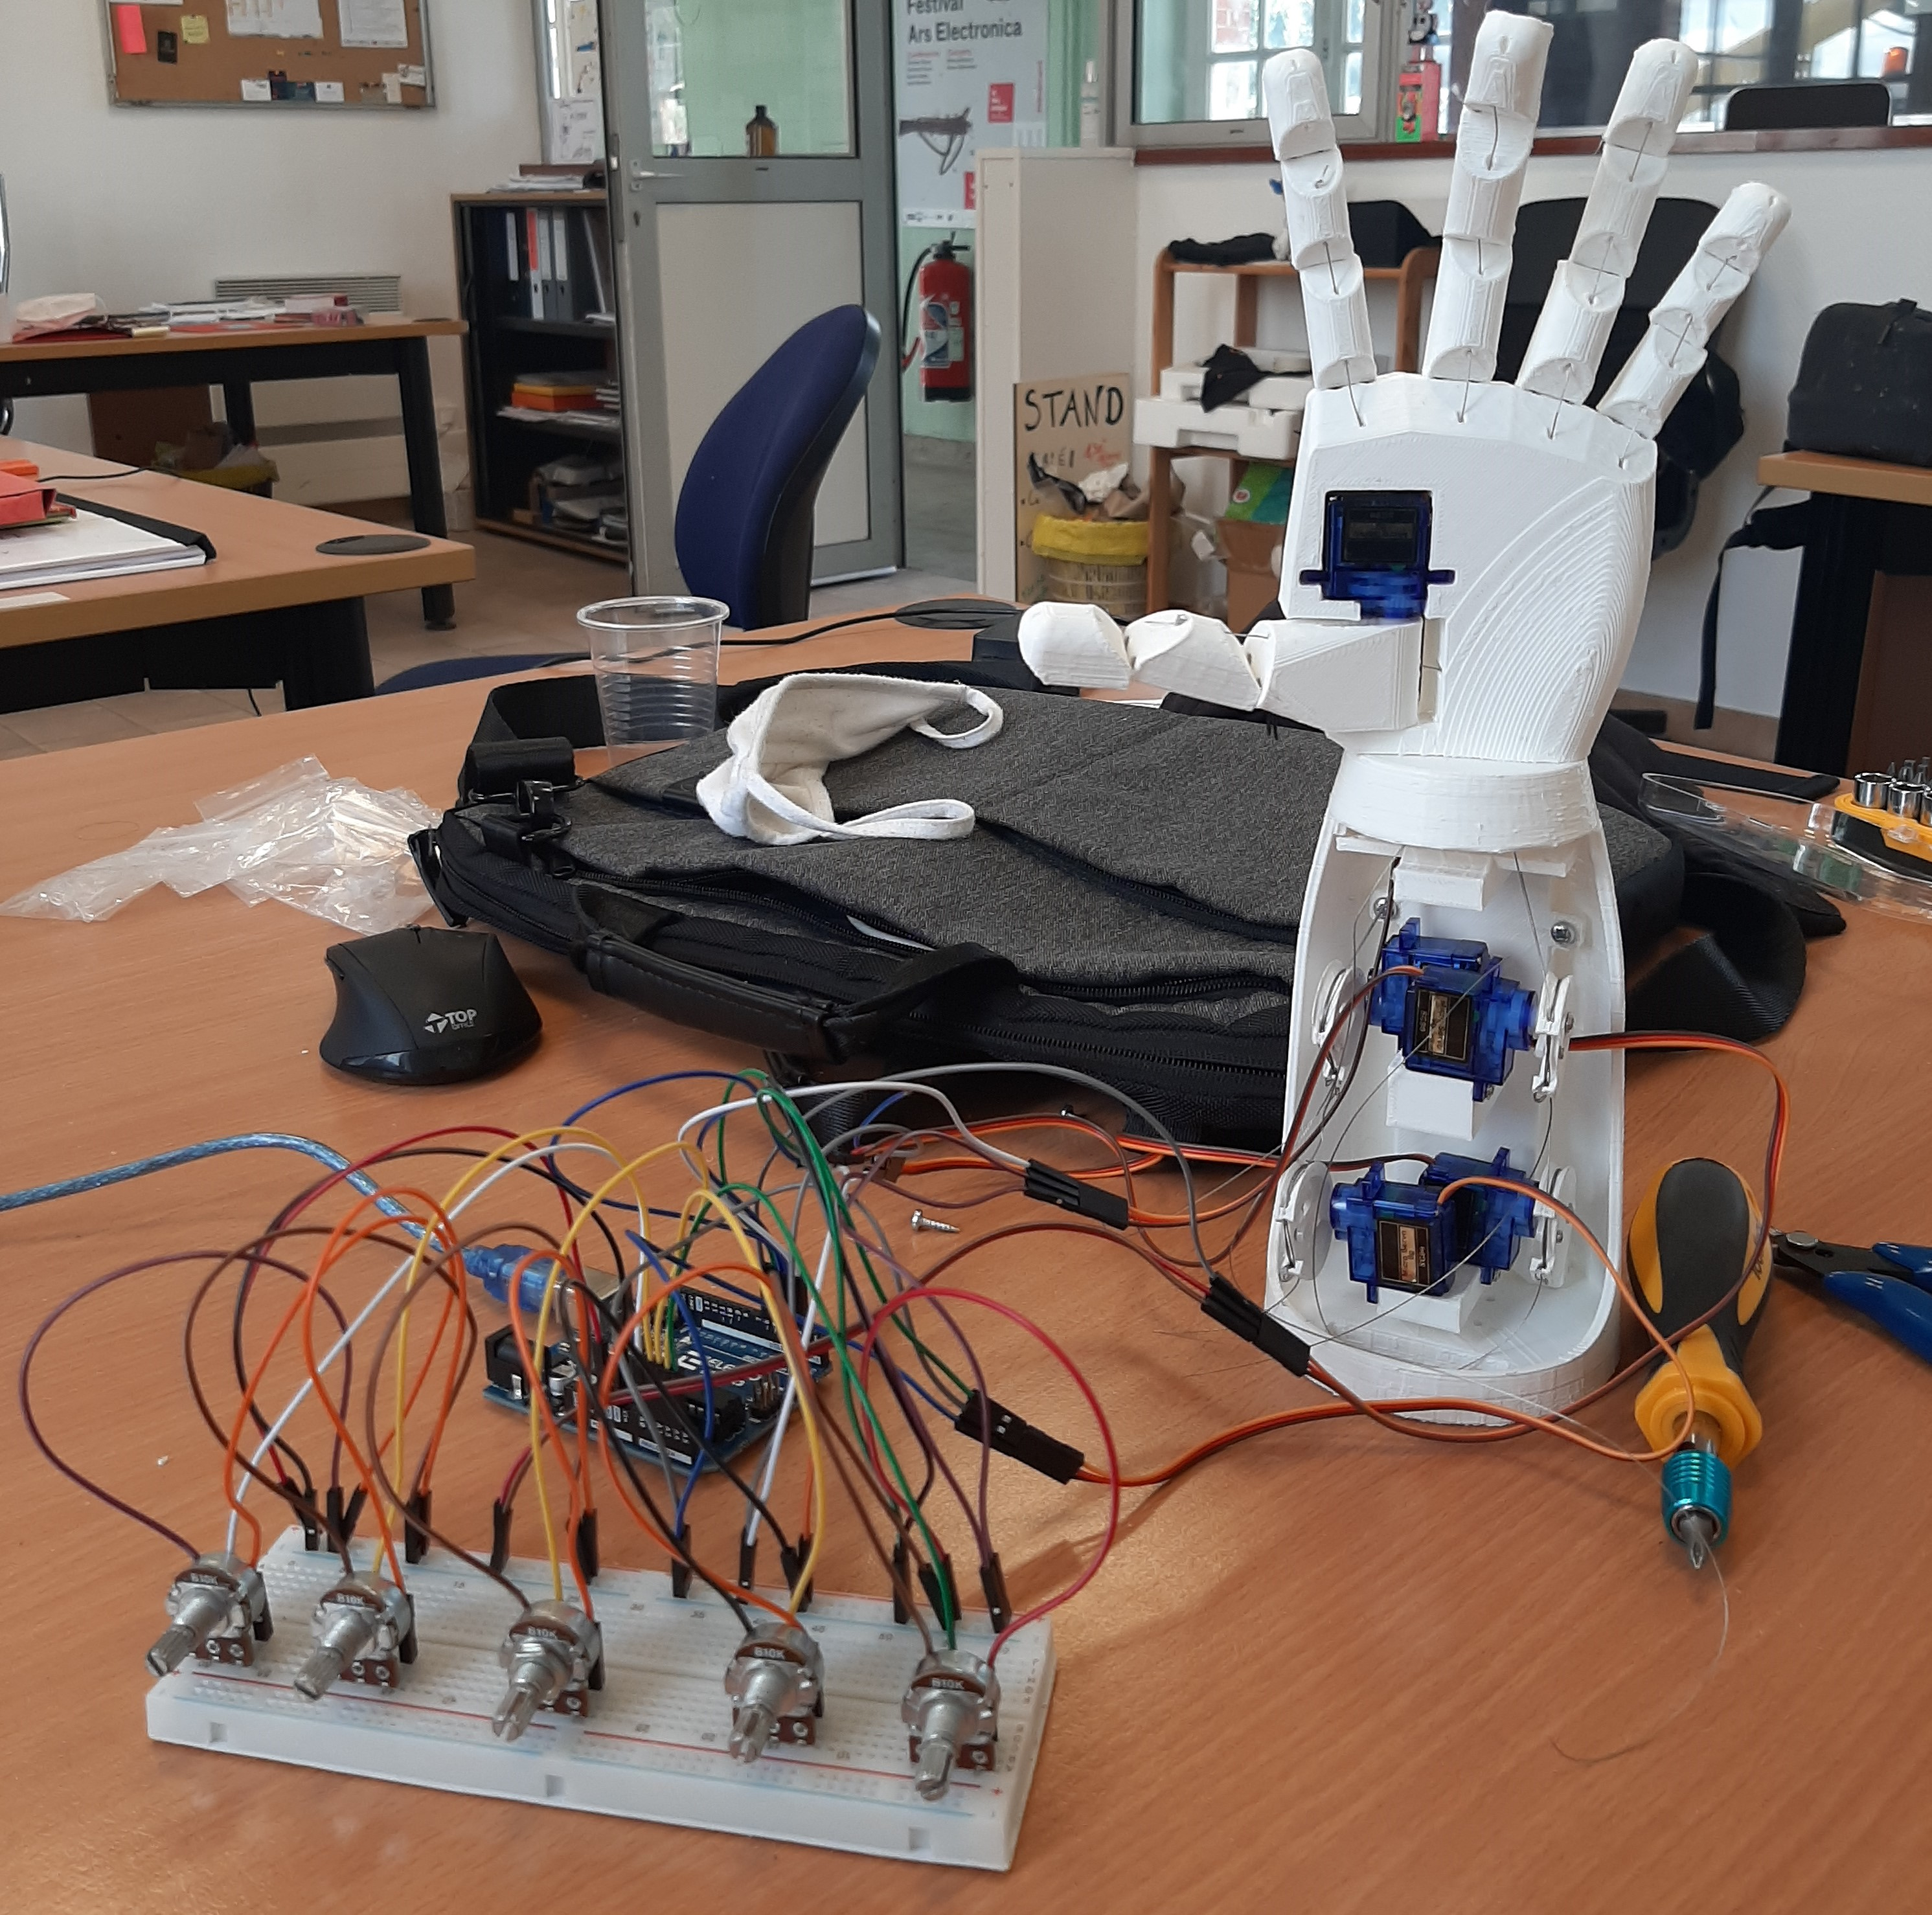
\includegraphics[width=300pt]{Déroulé/Jour_3/Montage de la main/étape6.jpg}
    \caption[\'Etape 6]{Montage de la main - \'Etape 6}
    \label{fig:my_label}
\end{figure}

\end{flushleft}